\documentclass[a4paper,11pt]{article}

\usepackage[T1]{fontenc}
\usepackage{lmodern}
\usepackage{amsmath}
\usepackage{graphicx}
\setlength\abovecaptionskip{0.10ex}
\usepackage{titling}
\setlength{\droptitle}{-4cm}
\usepackage{fullpage}
\RequirePackage{graphicx}
\DeclareGraphicsExtensions{.pdf,.jpg,.png,.JPG}
\RequirePackage{float}

\newcommand{\InsertFig}[1]{
\begin{figure}[H]
\begin{center}
\includegraphics[width=.75\textwidth]{img/#1}
\end{center}
\end{figure}}
\newcommand{\InsertFigTitle}[2]{
\begin{figure}[H]
\caption{#2}
\begin{center}
\includegraphics[width=.75\textwidth]{img/#1}
\end{center}
\end{figure}}

\title{Rapport SY19 TP01 - Classification et melange}
\author{Thomas ABASSI \& Joan MOESCH}

\begin{document}
\maketitle

\noindent Le but de ce TP est la comprehension et l'utilisation de differentes methodes pour la classification  non supervisee. En effet, nous analyserons tout d'abord l'algorithme des centres mobiles a travers la fonction $kmeans$ de R. \\
Apres avoir apprecie les possibilites et les limites de cette methode, nous etudierons le modele de melanges grace aux algorithmes $EM$ et $CEM$. Cette etude portera sur des donnees synthetiques puis sur des donnees reelles et seront effectuees sur dans le cas monodimensionnel et multidimensionnel. \\

\section{La methode des Centres Mobiles}

\subsection{La fonction kmeans}
\noindent Nous utilisons la fonction R $kmeans$ avec un nombre de partition de K = 2,3 puis 4 . Voici les resultats obtenus : \\
\hspace{-2.5cm} \includegraphics[width=.55\textwidth]{Exo1/K2.pdf} \includegraphics[width=.5\textwidth]{Exo1/K3.pdf}
\begin{center} \includegraphics[width=.5\textwidth]{Exo1/K4.pdf} \end{center} 

\noindent Chaque couleur correspond aux vrais classes des donnees alors que les symboles designent respectivement les classes determinees par la methodes de K-means.\\
Nous remarquons que les resultats sont satisfaisants dans le cas ou le nombre de partition est egale au nombre de classe. Dans le cas contraire, une classe est typiquement scindee en 2 ou au contraire 2 classes sont fusionees. D'autre part, nous remarquons que les resultats varient sur plusieurs executions de la fonction. En effet cette derniere est trop dependante des premiers centres choisis en debut d'algorithme.\\
Il peut donc etre interessant de trouver une methode qui exercerait une moyenne des resultats de $kmeans$ et une methode qui nous indiquerait comment choisir le bon nombre de partition.


\subsection{Stabilite}
\noindent Afin d'evaluer la stabilite de la methode des centres mobiles nous ecrivons la fonction suivante : \\

\noindent intra <- function()

	res <- matrix( nrow=100, ncol=1);
	
	for( i in 1:100)
	
	\hspace{1cm} K <- kmeans(donneesnum, 3);
		
	\hspace{1cm}res[i,1] <- sum(Kwithinss);
		
	m <- min( res[,1])
	
	M <- max( res[,1])
	
	moy <- mean(res[,1])
	
	return (list(intra=res, min=m, max=M, avg =moy) );\\
	
\noindent Ainsi nous obtenons les resultats suivants : \\
$W_{min} = 78.85144$\\
$W_{max }= 142.7535$\\
$W_{moy} = 89.7148$ \\

\noindent Visuellement, le partitionnement est different a chaque execution de la methode k-means, certains sont meilleurs que d'autres.
La comparaison des valeurs min, moy et max de l'inertie intra classe confirme la grande variation de cette methode.

\subsection{Nombre de classes optimale}
\noindent Afin de selectionner le nombre de classes optimale, nous implementons en une fonction R la methode du coude : \\

\noindent inertie <- function()

	res <- matrix(nrow=4, ncol=1);
	
	for(j in 2:5)
	
	\hspace{1cm} for( i in 1:100 )

	\hspace{1.5cm} K = kmeans(donneesnum, j);
	
	\hspace{1.5cm} res[j] = sum(Kwithinss);

	return(res);\\

\begin{center}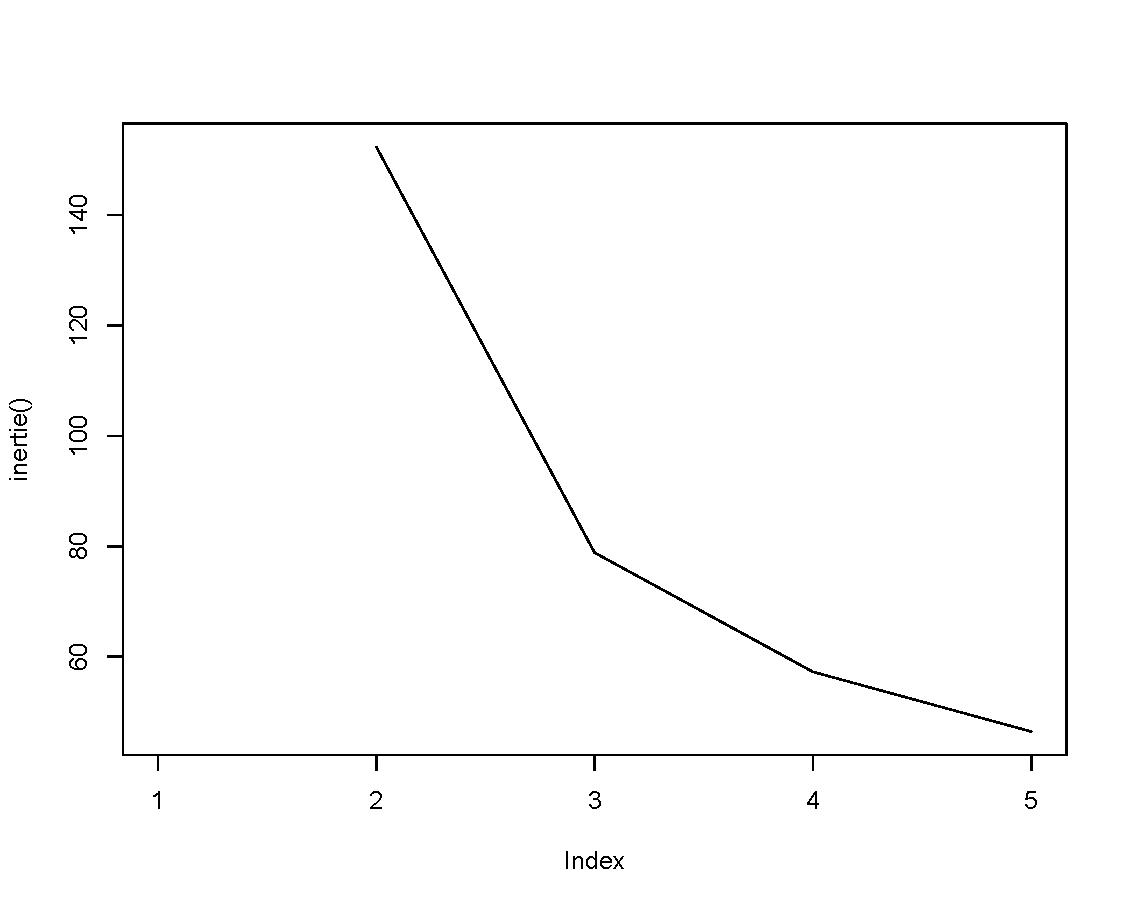
\includegraphics[width=.6\textwidth]{Exo1/coude.pdf} \end{center}
\noindent La methode du coude nous permet ainsi de visualiser que $k=3$ classes est le nombre de classes optimal pour la classification. En effet, tant que la diminution de l'intertie intraclasse est importante, on continue d'augmenter le nombre de classes jusqu'a n'obtenir que de plus petites variations. L'abcisse de ce changement de variations est le nombre optimal de partitionnement.

\subsection{Comparaison avec la partition reelle}

\noindent L'inertie intra classe correspond a la variance pour chaque classe (sans le $\frac{1}{nk}$)
Pour 1 classe donnee, cette inertie est donc la variance du nuage multiplie par (n-1) car VAR est variance empirique corrigee sous R.\\

\noindent setosa = iris[1:50,1:4]\\
w1 = sum( diag(49 * var(setosa)) ) = 15.151\\

\noindent versicolor = iris[51:100,1:4]\\
w2 = sum( diag(49 * var(versicolor)) ) = 30.6164\\

\noindent virginia = iris[101:150,1:4]\\
w3 = sum( diag(49 * var(virginia)) ) = 43.53\\

\noindent l'inertie totale est donc donnee par : $w = (w1 + w2 + w3) = 89.2974$

\noindent On avait $W_{moy} = 89.7148$ et $W_{min} = 78.85144$, l'inertie reelle est sans surprise inferieure a celle trouvee par les kmeans. \\

\noindent Si on calcule les inertie intra-classe des partitions trouvees par la methode des K-means, on obtient :  \\

$W_1 = 26.51234, W_2 = 33.21364, W_3 =  36.37902$\\

\noindent Ces valeurs sont proches des inerties intra-classe reelles. Elles peuvent etre inferieures car la methode des k-means peut parfois trouver de meilleures classes que les reelles.

\section{Algorithmes EM et CEM dans le cas monodimensionnel}
\subsection{Donnees synthetiques}
\subsubsection{Implementation des algorithmes EM et CEM}
 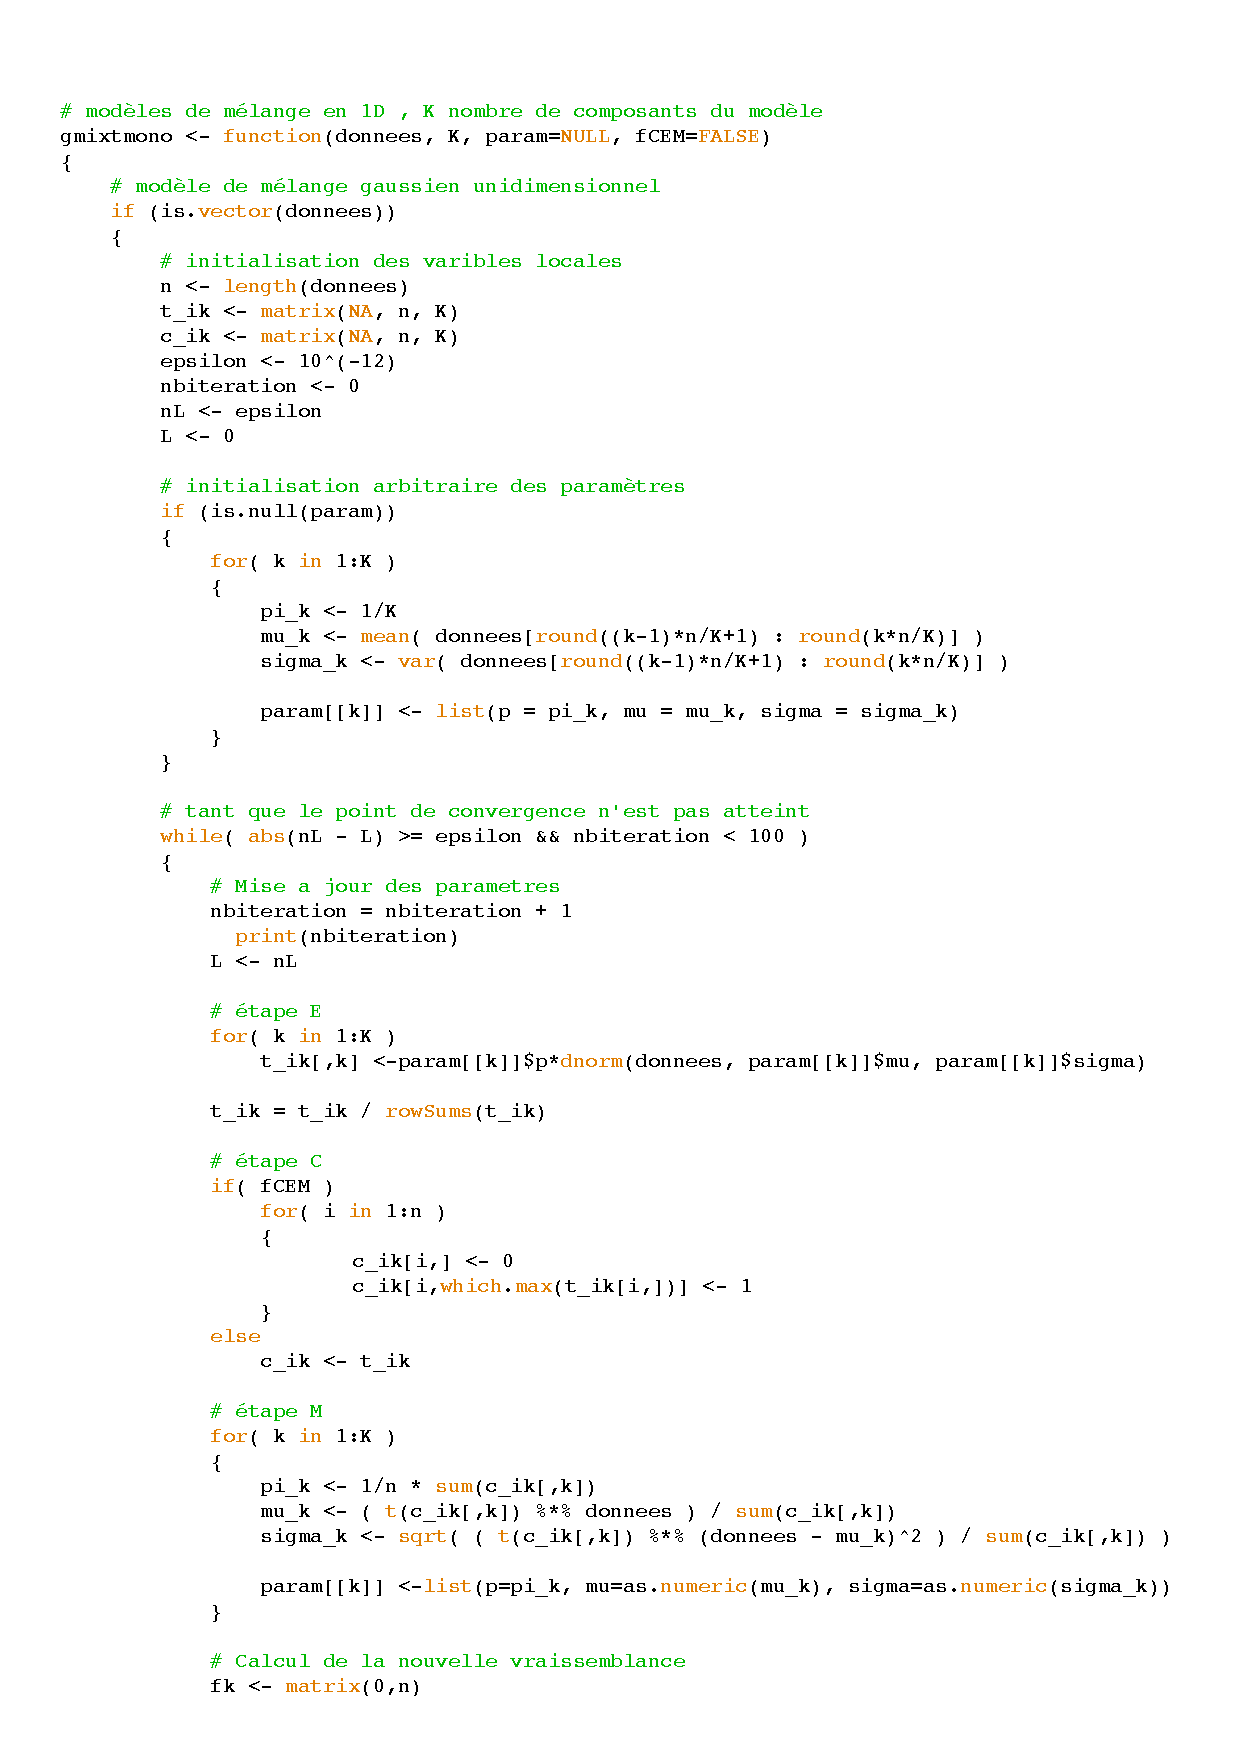
\includegraphics[width=0.9\textwidth]{Exo2/EM_CEM.pdf} \\
  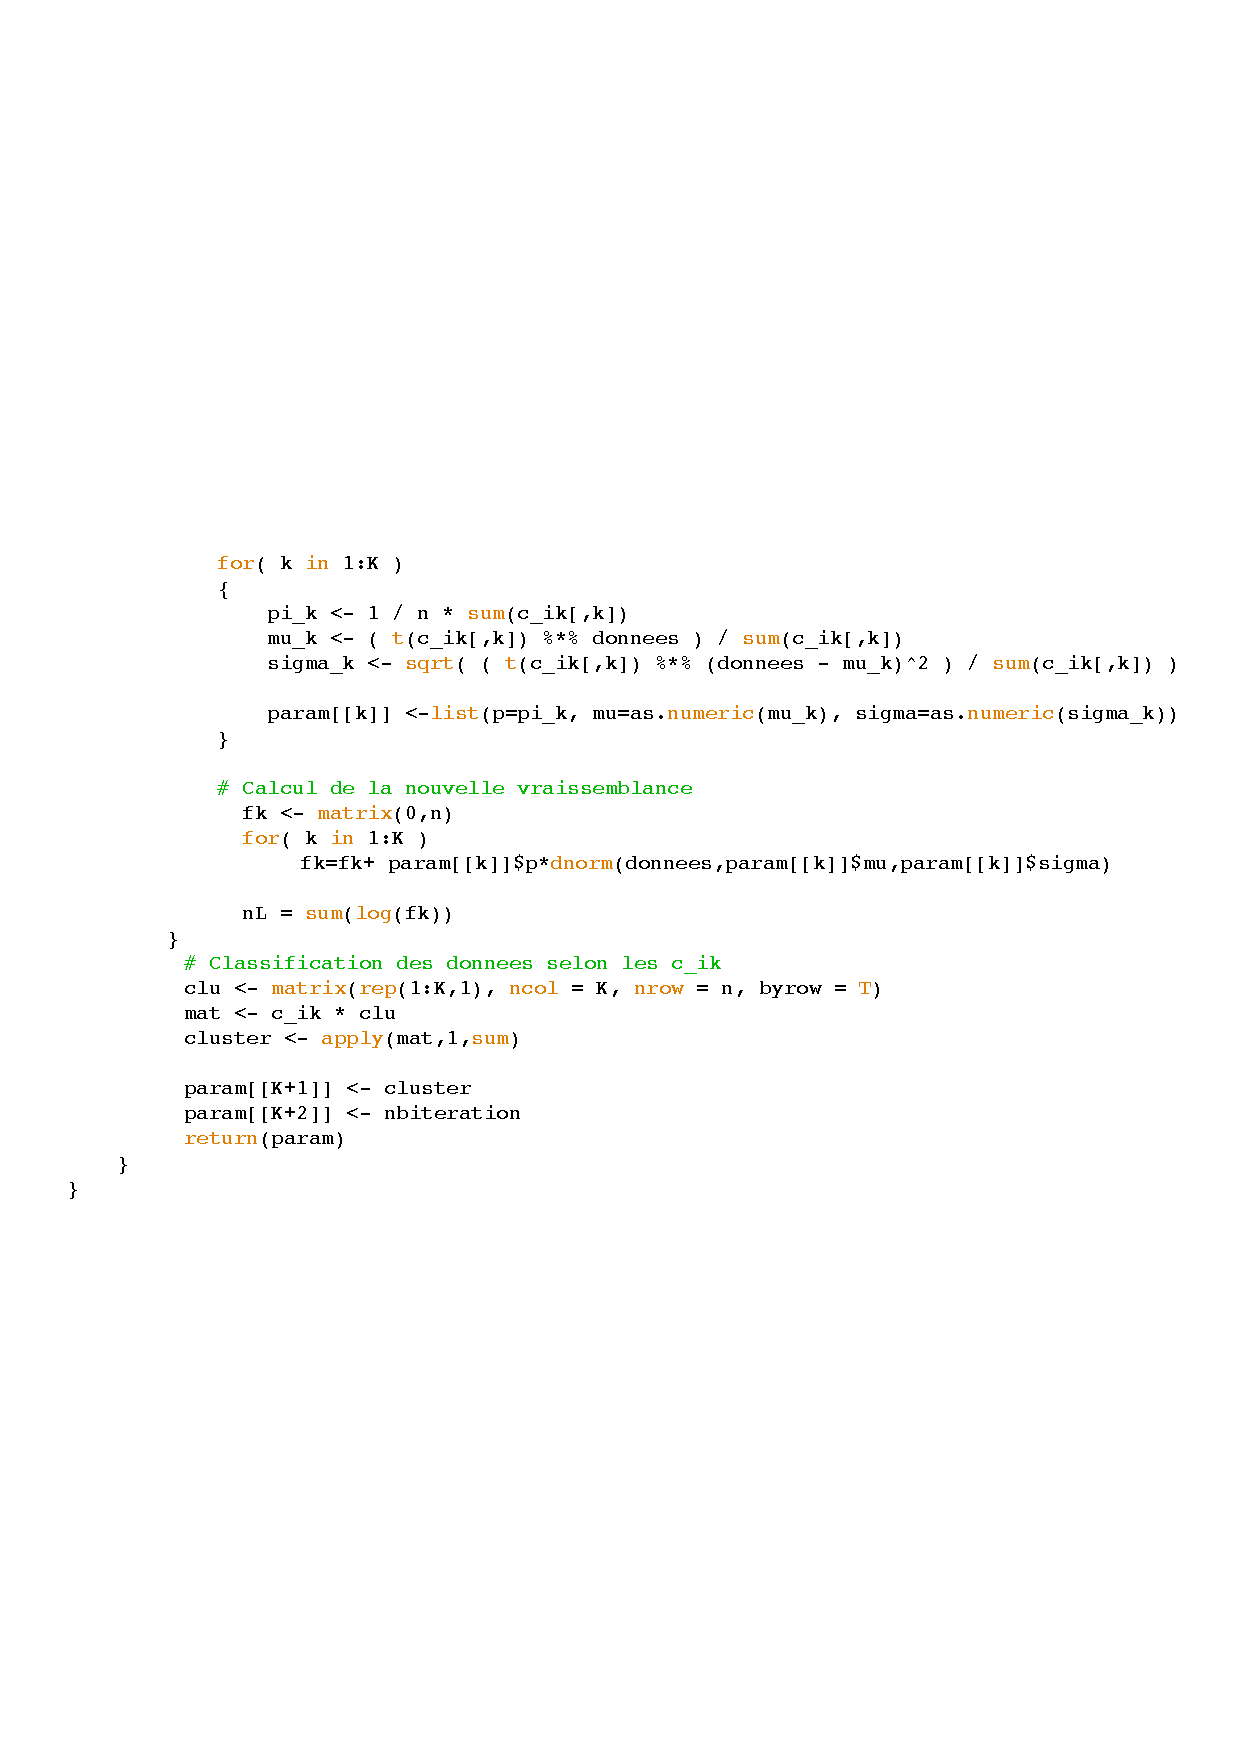
\includegraphics[width=0.9\textwidth]{Exo2/EM_CEM2.pdf}


\subsubsection{Comparaison des algorithmes EM et CEM}
\noindent A partir des donnees synthetiques $x<-c(rnorm(1000),rnorm(1000,mean=6,sd=5))$, nous obtenons les resultats suivants : \\

\noindent EM <- gmixtmono(x,2) : Avec une precision de $10^{-12}$, l'algorithme EM termine en 49 iterations : \\
$\pi_1 = 0.5051534$ \hspace{0.5cm} $\pi_2 = 0.4948466$\\
$\mu_1 = 0.07185754$ \hspace{0.33cm}  $\mu_2 = 6.28883$\\
$\sigma_1 = 1.001384$ \hspace{0.67cm}  $\sigma_2 = 4.915321$\\

\noindent CEM <- gmixtmono(x,2,NULL,T) : Avec une precision de $10^{-12}$, l'algorithme CEM termine en 10 iterations : \\
$\pi_1 = 0.6045$ \hspace{0.9cm}  $\pi_2 = 0.3955$\\
$\mu_1 = 0.1126677$ \hspace{0.3cm} $\mu_2 = 7.78811$\\
$\sigma_1 = 1.121608$ \hspace{0.48cm} $\sigma_2 = 4.289954$\\

\noindent D'une maniere generale, ces algorithmes retrouvent de maniere satisifaisante les  proportions ainsi que les parametres des 2 melanges gaussiens.\\
\noindent En comparant, on se rend compte que l'algorithme EM donne de meilleurs resulats que CEM. En effet, la moyenne et la variance trouvees par ce dernier est plus proche de la realite (0 et 1, 5 et 6).\\
\noindent Cependant, il est a noter que pour des resultats quand meme bons, l'algorithme CEM converge bien plus rapidement (10 iterations contre 49).

\subsubsection{Comparaison des algorithmes EM, CEM et Kmeans}
\noindent Afin de comparer les classifications entre kmeans, EM et CEM, nous ecrivons :

$EM <- gmixtmono(donnnees, 2)$

$CEM <- gmixtmono(donnnees, 2, NULL, T)$

$k <- kmeans(donnees, 2)$

\begin{center} 
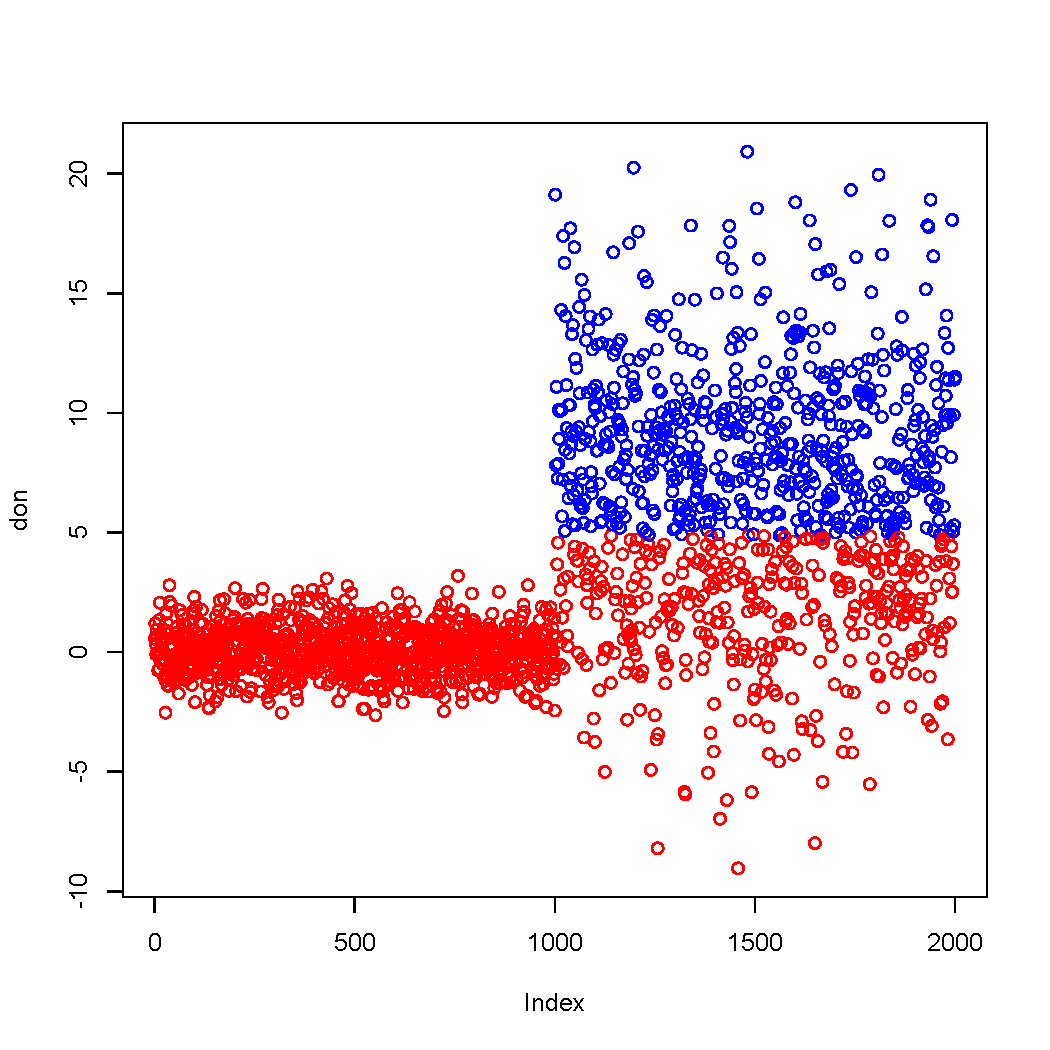
\includegraphics[width=.5\textwidth]{Exo2/kmeans.pdf}\\
$plot(donnees, col=c("red","blue")[kcluster])$
\end{center}
\hspace{-0.2cm} 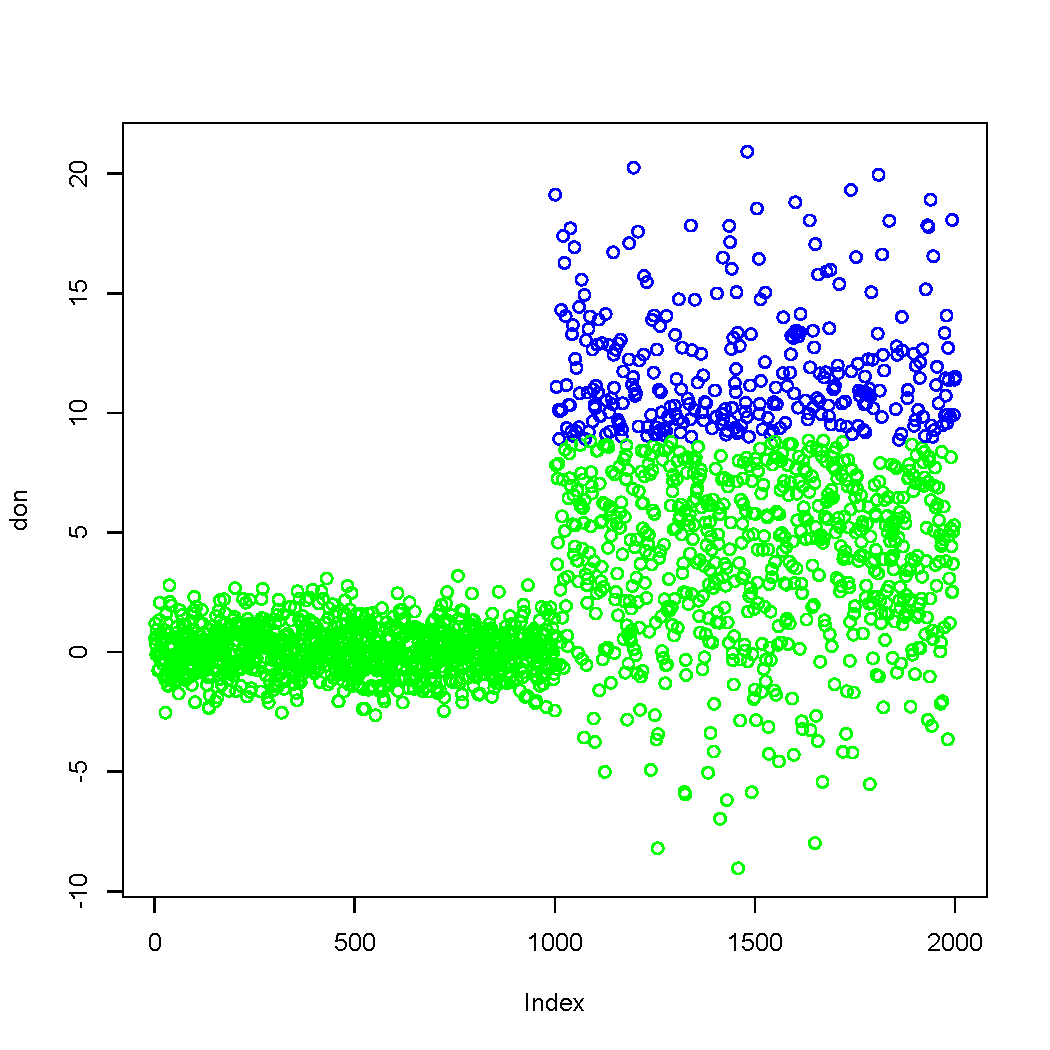
\includegraphics[width=.5\textwidth]{Exo2/EM.pdf} \hspace{0.3cm} 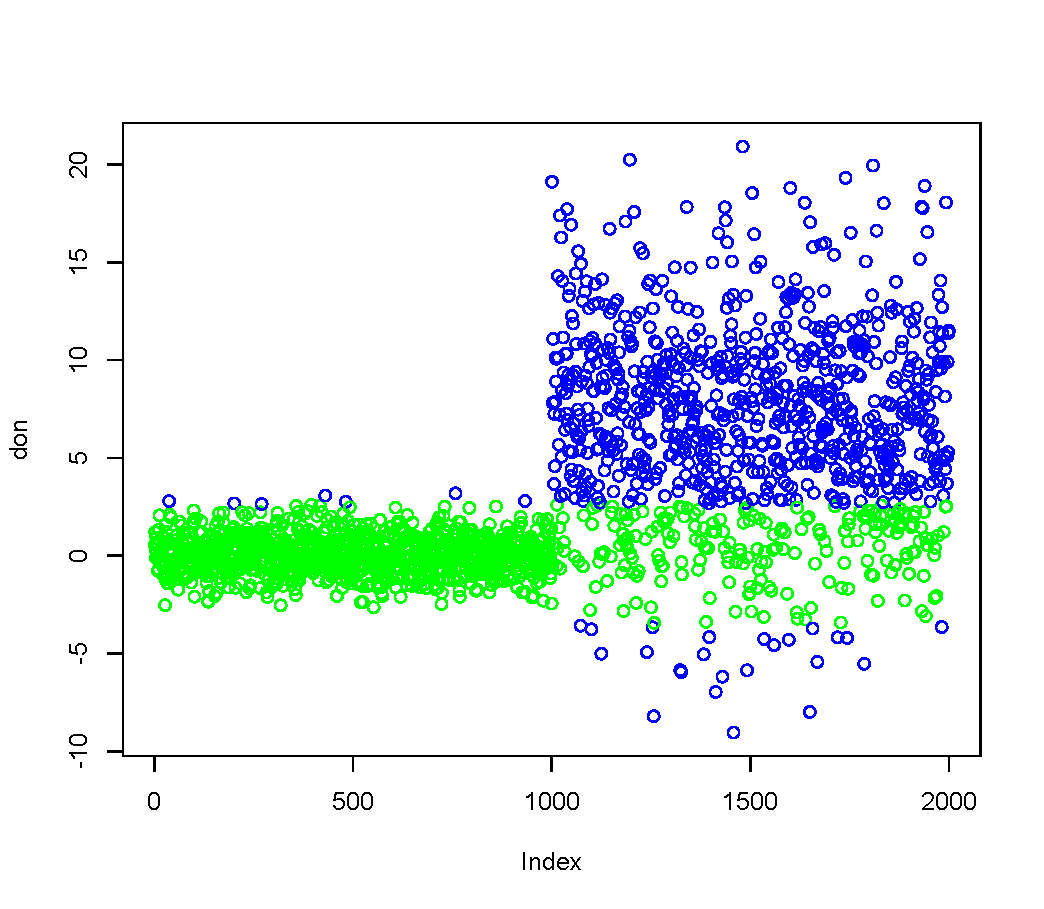
\includegraphics[width=.6\textwidth]{Exo2/CEM.pdf} \\
$plot(donnees, col=c("red","blue")[EM[[3]]])$ \hspace{1.6cm} $plot(donnees, col=c("red","blue")[CEM[[3]]])$ \\

\noindent Le premier graphique (en rouge) represente la classification effectuee par $kmeans$. Les 2 autres (en vert) representent respectivement les classifications faites par EM et CEM.\\
Ainsi, on remarque que la classification selon l'algorithme CEM est la meilleure. En effet, la methode des $kmeans$ donne une separation en x = 5 des donnees. Les donnees inferieures a cette droite seront du 1er melange et ceux au dessus de la droite du 2eme. De la meme maniere EM separe les donnees en x = 8.\\

En revanche, la classification CEM regroupe les donnees en 0 (plus ou moins 2) et le reste des donnees. Cette separation se rapproche bien plus de notre melange d'origine : un groupe de moyenne 0 avec une variance reduite (1) et un autre de 5 avec une variance plus grande (6).

\subsection{Donnees reelles}
\subsubsection{Application des algorithmes EM et CEM pour la classification de pixels}
\noindent Afin de pouvoir utiliser nos algorithmes EM et CEM, nous transformons la matrice d'image lena en un vecteur, puis nous appliquons nos differents algorithmes pour un modele de K = 4 melanges :

$y <- immat2imvec(lena)$

$EM <- gmixtmono(yvec,4)$ et $CEM <- gmixtmono(yvec,4,NULL,T)$ \\

\noindent Nous transformons ensuite ces resultats en matrice a 2 dimensions pour les afficher :

$imEM <- imvec2immat(EM[[5]])$ et $imCEM <- imvec2immat(EM[[5]])$

$ implotbw(imEM) $ et $ implotbw(imCEM) $ \\

\noindent Nous n'avons pas pu terminer car des NaN aparraissent dans les algorithmes et les donn�es obtenues ne nous permettent pas de tracer les images. Avec les kmeans, nous obtenons :


\begin{figure}[H]
\begin{center}
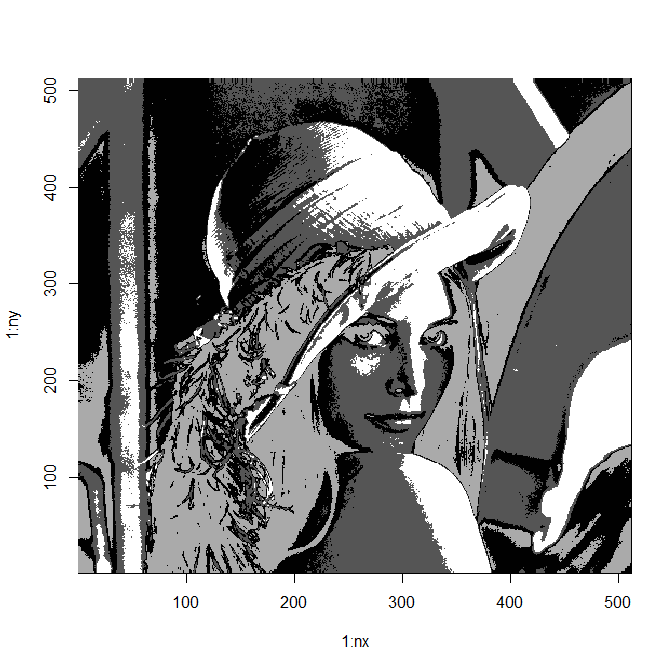
\includegraphics[width=.6\textwidth]{Exo2/lenaKMeans.png}
\end{center}
\end{figure}

\section{Algorithmes EM et CEM dans le cas multidimensionnel}

\subsection{Implementation des algorithmes EM et CEM}

\noindent Ces algorithmes r�p�tent les �tapes `Expectation', `Maximisation' ou `Expectation', `Classification', `Maximisation' Les algorithmes s'arr�tent lorsque la variation de la log vraisemblance passe au dessous d'un seuil ou au bout d'un certain nombre d'it�rations.

\noindent L'impl�mentation de ces algorithmes fait 130 lignes de codes. Le code ne sera donc pas rapport� ici, n�anmoins les points cl�s sont :\\

\noindent Calcul de $t_{ik}$ : $t_{ik} = \frac{\Pi_{k}\varphi(x_{i}\mu_{k}\Sigma_{k})}{\sum_{l}{\Pi_{l}\varphi(x_{i}\mu_{l}\Sigma_{l})}}$

\noindent Calcul de $\Pi_{k}$ : $\Pi_{k} = \frac{\sum\limits^{n}_{i=1}t_{ik}}{n}$

\noindent Calcul de $\mu_{k}$ : $\mu_{k} = \frac{\sum\limits^{n}_{i=1}t_{ik}x_{i}}{\sum\limits^{n}_{i=1}t_{ik}}$

\noindent Calcul de $\Sigma_{k}$ : $\Sigma_{k} = \frac{\sum\limits^{n}_{i=1}t_{ik}(x_{i}-\mu_{k})(x_{i}-\mu_{k})^T}{\sum\limits^{n}_{i=1}t_{ik}}$

\noindent Calcul de la log vraisemblance : $L_{C} = \sum \limits_{i,k}z_{i,k}log(\Pi_{k}\phi(x_{i}\mu_{k}\Sigma_{k}))$

\subsection{Premiere comparaison entre l'algorithme des centres mobiles, l'algorithme EM, et l'algorithme CEM}

\noindent On peut remarquer que l'algorithme CEM converge plus vite que l'algorithme EM ( EM : 49 iterations pour atteindre une variation de la log vraisemblance inf�rieure a $10^{-6}$ avec 3 classes. CEM : 12 it�rations pour le m�me epsilon avec le m�me nombre de classes)

\noindent On peut remarquer que l'algorithme CEM donne des r�sultats similaires a l'algorithme des centres mobiles. Cela peut s'expliquer par le fait que l'algorithme des centres mobiles correspond � un cas particulier simple de l'algorithme CEM.\\

\noindent Si les partitions obtenues grace � CEM et les centres mobiles d'une part et EM d'autre part sont differentes pour $K=2$, en revanche pour $K=3$ et $K=4$, les partitions sont a peu pr�s similaires. Nous avons stopp� l'algorithme EM � 50 iterations pour $K=2$. Peut �tre qu'avec un plus grand nombre d'iterations, nous aurions obtenu des partitions plus proches.

\noindent La partition en 4 classes semble �tre la meilleure, m�me si la partition initiale etait de 3 classes. Les 3 classes initiales ont bien �t� reconstruites et une 4eme classe comprend les elements 'g�nants'.\\

\noindent Ci-dessous, la division en 4 classes obtenue � partir de l'algorithme CEM.

\begin{figure}[H]
\begin{center}
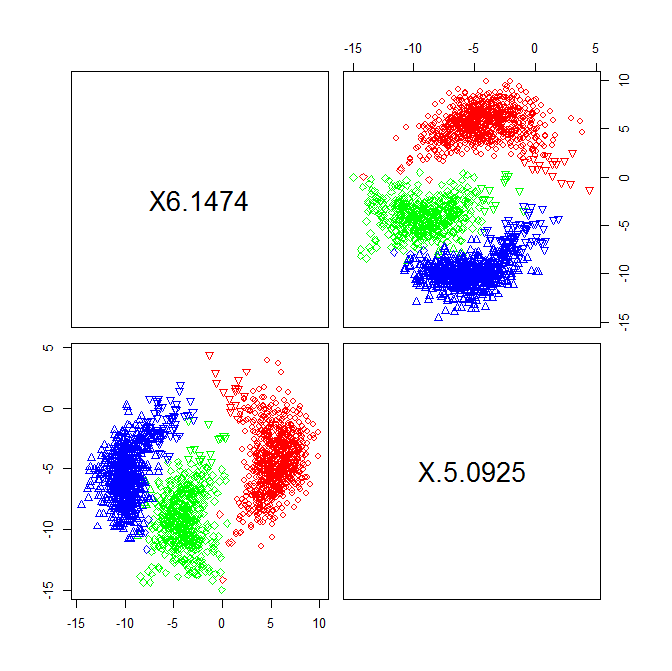
\includegraphics[width=.5\textwidth]{Exo3/4classes.png}
\end{center}
\end{figure}

\subsection{Seconde comparaison entre l'algorithme des centres mobiles, l'algorithme EM, et l'algorithme CEM}

\noindent Ces methodes donnent des resultats a peu pres similaires. Les partitions obtenues respectent bien la partition originale. Ci-dessous, les differentes formes representent les differentes classes et quant au couleurs, dans la premiere figure
elles sont en fonction de l'�spece r�elle et dans la seconde figure elles sont fonction du sexe r�el.

\begin{figure}[H]
\begin{center}
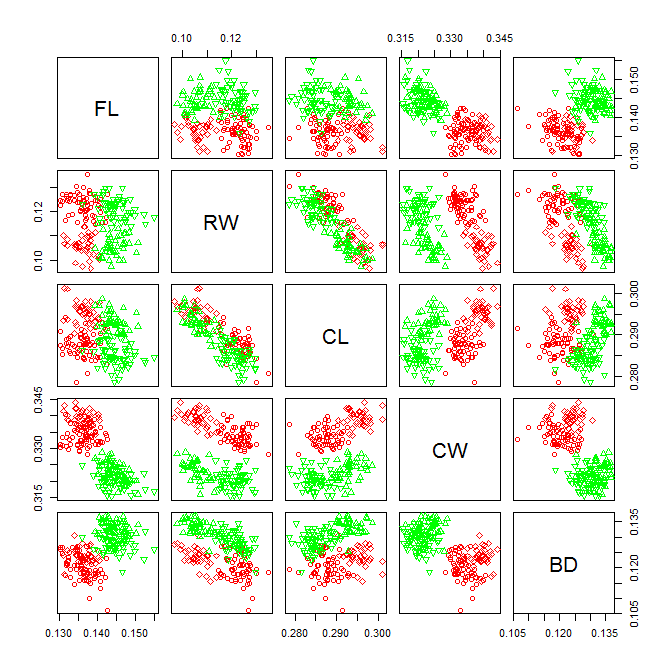
\includegraphics[width=.55\textwidth]{Exo3/especeCrabes.png}
\end{center}
\end{figure}
\begin{figure}[H]
\begin{center}
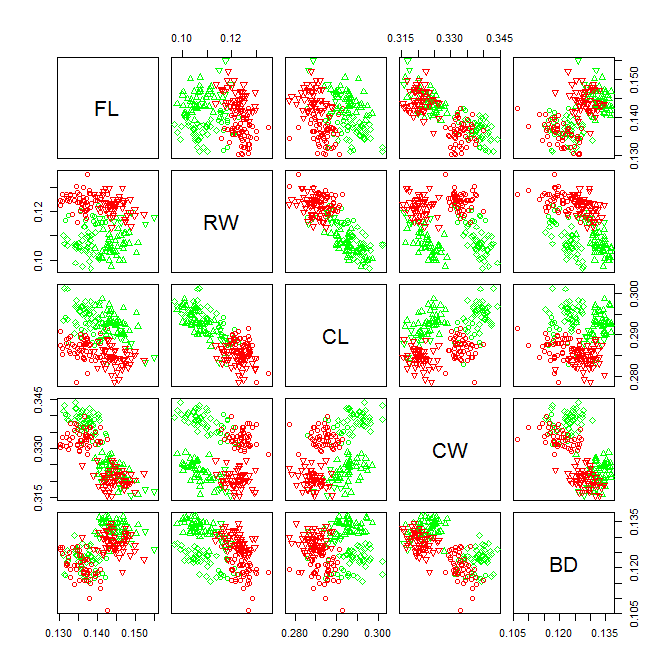
\includegraphics[width=.55\textwidth]{Exo3/sexeCrabes.png}
\end{center}
\end{figure}


\end{document}